% ============================================================
% CHƯƠNG 2: CÁC CÔNG TRÌNH LIÊN QUAN VÀ CƠ SỞ LÝ THUYẾT
% ============================================================
\chapter{CÁC CÔNG TRÌNH LIÊN QUAN VÀ CƠ SỞ LÝ THUYẾT}
\label{Chapter2}

Chương này gồm hai phần chính. Phần đầu điểm lại các hướng nghiên cứu có liên quan đến phân đoạn ảnh y khoa, nhất là các mô hình tự động, các phương pháp phân đoạn tương tác dựa trên CNN và các mô hình nền tảng có dùng câu nhắc. Từ phần này, khóa luận rút ra khoảng trống nghiên cứu cần hướng tới. Phần sau trình bày các cơ sở lý thuyết cần dùng như U-Net, cơ chế chú ý, cách biểu diễn câu nhắc trực quan và các chỉ số đánh giá mô hình.

% ------------------------------------------------------------
\section{Các công trình liên quan}
\label{sec:related_work}
% ------------------------------------------------------------

\subsection{Phân đoạn ảnh y khoa tự động}

Trước khi U-Net trở thành một kiến trúc gần như quen mặt trong phân đoạn ảnh y khoa, các phương pháp phân đoạn ngữ nghĩa bằng học sâu đã đi theo nhiều hướng khác nhau. Có thể kể đến các mạng tích chập thuần như FCN~\cite{long2015fcn}, các mô hình mã hóa--giải mã như SegNet~\cite{badrinarayanan2017segnet}, hoặc các kiến trúc khai thác ngữ cảnh đa tỉ lệ như DeepLabv3+~\cite{chen2018deeplabv3plus}. Có thể xem đây là những bước nền để các mô hình phân đoạn về sau phát triển mạnh hơn~\cite{minaee2021survey}.

U-Net~\cite{ronneberger2015unet} là một trong những kiến trúc phổ biến nhất của phân đoạn ảnh y khoa. Mô hình có dạng mã hóa--giải mã đối xứng và dùng các kết nối tắt để giữ lại thông tin vị trí từ các tầng nông trong lúc vẫn học được đặc trưng ngữ nghĩa ở các tầng sâu. Thiết kế này hợp với dữ liệu y khoa, vốn thường không có quá nhiều ảnh được gán nhãn phân đoạn.

Attention U-Net~\cite{oktay2018attentionunet} phát triển tiếp từ U-Net bằng cách thêm các Cổng chú ý ở các kết nối tắt. Ý tưởng ở đây là mô hình học cách ưu tiên những vùng quan trọng hơn trước khi đặc trưng được chuyển sang bộ giải mã. Nhờ vậy, mô hình có thể tập trung tốt hơn vào cấu trúc cần phân đoạn mà không cần thêm một mạng định vị riêng.

Tuy nhiên, ở dạng gốc thì cả U-Net lẫn Attention U-Net đều là các mô hình tự động, nghĩa là chỉ nhận ảnh đầu vào và phải tự tìm vùng cần phân đoạn. Với ảnh X-quang xương, đây là một yêu cầu không hề nhẹ vì tổn thương có thể nhỏ, mờ hoặc nằm trong vùng nhiều cấu trúc chồng lấp. Ngoài ra, bác sĩ chẩn đoán ảnh cũng khó can thiệp để hướng mô hình tập trung vào một vùng cụ thể tại thời điểm suy luận.

Sau U-Net, nhiều biến thể được đề xuất để cải thiện hiệu năng hoặc giảm công sức tinh chỉnh thủ công. Chẳng hạn, UNet++~\cite{zhou2018unetplusplus} thiết kế lại các đường nối tắt theo dạng lồng nhau để thu hẹp khoảng cách ngữ nghĩa giữa bộ mã hóa và bộ giải mã, còn nnU-Net~\cite{isensee2021nnunet} nhấn mạnh rằng hiệu năng trong ảnh y khoa không chỉ đến từ kiến trúc mạng mà còn đến từ quy trình cấu hình, tiền xử lý và hậu xử lý. Điều này cũng nhắc rằng bài toán phân đoạn y khoa không phụ thuộc vào một mô-đun đơn lẻ.

% ------------------------------------------------------------
\subsection{Phân đoạn tương tác dựa trên CNN}

Phân đoạn tương tác cho phép bác sĩ cung cấp thông tin bổ sung như điểm bấm~\cite{xu2016deepinteractive}, nét vẽ hoặc hộp giới hạn để hướng mô hình đến vùng cần xử lý. Thông tin tương tác thường được chuyển thành một hoặc nhiều bản đồ không gian và đưa vào CNN cùng với ảnh.

Các phương pháp tương tác ban đầu thường khai thác tín hiệu bác sĩ ở dạng điểm bấm hoặc nét vẽ. Deep Interactive Object Selection~\cite{xu2016deepinteractive} là một ví dụ sớm cho thấy chỉ với những tương tác đơn giản, nếu mã hóa phù hợp thành bản đồ khoảng cách rồi đưa vào CNN thì chất lượng mặt nạ có thể tăng đáng kể. Trong ảnh y khoa, DeepIGeoS~\cite{wang2019deepigeos} là một ví dụ tiêu biểu. Cách làm của phương pháp này là tạo một phân đoạn ban đầu, sau đó dùng thêm tương tác bác sĩ để tinh chỉnh lại những vùng còn sai.

Nhìn chung, các phương pháp này cho thấy tương tác của bác sĩ hoàn toàn có thể đổi thành bản đồ hai chiều và đưa trực tiếp vào CNN. Dù vậy, nếu chỉ ghép bản đồ đó ở đầu vào thì chưa chắc thông tin định hướng còn rõ ở các tầng sâu hơn của mạng. Đây cũng là một lý do để khóa luận đi tiếp theo hướng tích hợp câu nhắc sâu hơn vào quá trình mã hóa và giải mã đặc trưng.

% ------------------------------------------------------------
\subsection{Mô hình nền tảng dựa trên câu nhắc}

Segment Anything Model (SAM)~\cite{2023-SAM-Kirillov} là mô hình nền tảng cho phân đoạn ảnh tự nhiên, hỗ trợ nhiều dạng câu nhắc như điểm, hộp giới hạn và mặt nạ. Kiến trúc gồm bộ mã hóa ảnh, bộ mã hóa câu nhắc và bộ giải mã mặt nạ. Cách tổ chức này cho phép một mô hình thực hiện nhiều tác vụ phân đoạn mà không cần thiết kế lại kiến trúc cho từng loại đối tượng.

Do ban đầu được huấn luyện chủ yếu trên ảnh tự nhiên, SAM có thể gặp khó khăn khi đem dùng trực tiếp cho ảnh y khoa. Vì vậy, SAM-Med2D~\cite{2023-SAMMed2D-Cheng} được phát triển để thích nghi SAM với ảnh y khoa 2D. Mô hình này bổ sung các lớp thích ứng và được huấn luyện trên một tập dữ liệu y khoa rất lớn gồm khoảng 4,6 triệu ảnh và 19,7 triệu mặt nạ. Một hướng tương tự là MedSAM~\cite{ma2024medsam}. Trong khóa luận này, SAM-Med2D được chọn làm mô hình đối sánh chính vì nó phù hợp hơn với dữ liệu 2D và hỗ trợ tinh chỉnh trực tiếp trên tập X-quang xương.

SAM-Med2D tiếp nhận câu nhắc thông qua bộ mã hóa riêng và kết hợp biểu diễn câu nhắc với đặc trưng ảnh để sinh mặt nạ. Trong khóa luận, hộp giới hạn được sử dụng làm câu nhắc nhằm bảo đảm điều kiện so sánh thống nhất với PGA-UNet.

\begin{figure}[htbp]
    \centering
    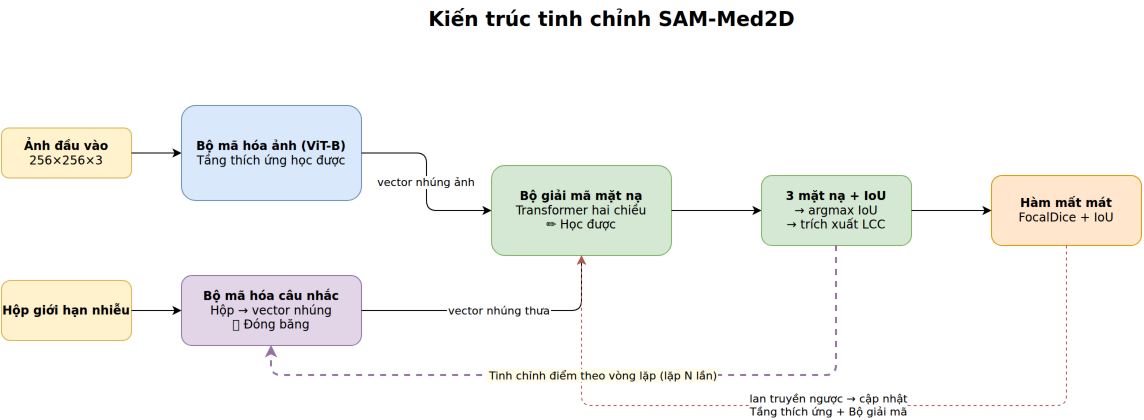
\includegraphics[width=0.98\textwidth]{images/arch_sammed2d.png}
    \caption{Kiến trúc SAM-Med2D với bộ mã hóa ảnh, bộ mã hóa câu nhắc, bộ giải mã mặt nạ và các lớp adapter thích ứng~\cite{2023-SAMMed2D-Cheng}.}
    \label{fig:sammed2d_architecture}
\end{figure}

SAM-Med2D có lợi thế là thừa hưởng kiến thức từ tiền huấn luyện trên lượng dữ liệu y khoa lớn, nhưng đổi lại kiến trúc cũng nặng hơn hẳn so với một CNN chuyên biệt. Trong thực nghiệm của khóa luận, SAM-Med2D được chạy ở độ phân giải $256\times256$, còn PGA-UNet được đánh giá ở cả $256\times256$ và $512\times512$. Vì vậy, ở Chương~\ref{Chapter4}, khóa luận có thêm các phép so sánh cùng độ phân giải để giảm bớt ảnh hưởng của khác biệt đầu vào.

Song song với SAM, nhiều công trình gần đây còn khảo sát khả năng kết hợp Transformer với phân đoạn y khoa. ViT~\cite{dosovitskiy2021vit} và Swin Transformer~\cite{liu2021swin} mở ra hướng biểu diễn dựa trên cơ chế chú ý toàn cục hoặc phân cấp; từ đó, các mô hình như TransUNet~\cite{chen2021transunet}, Swin-Unet~\cite{cao2022swinunet} được đề xuất cho nhiều tác vụ phân đoạn y khoa. Dù thường đạt hiệu năng cạnh tranh, các mô hình này cũng có xu hướng đòi hỏi tài nguyên tính toán và cấu hình huấn luyện phức tạp hơn so với các CNN gọn nhẹ.

% ------------------------------------------------------------
\subsection{Khoảng trống nghiên cứu}

Từ phần khảo sát ở trên có thể thấy mỗi hướng đều có điểm mạnh và điểm hạn chế riêng. U-Net và Attention U-Net gọn và quen thuộc nhưng ở dạng gốc thì không nhận câu nhắc. Các phương pháp tương tác dựa trên CNN có thể dùng bản đồ không gian, nhưng thường chỉ ghép tín hiệu này ở đầu vào hoặc ở một bước tinh chỉnh nào đó. Trong khi đó, SAM-Med2D nhận được nhiều loại câu nhắc và có lợi thế tiền huấn luyện quy mô lớn, nhưng chi phí tính toán cũng cao hơn.

Từ khoảng trống đó, khóa luận hướng đến một mô hình CNN tương đối nhẹ, có thể nhận trực tiếp hộp giới hạn và giữ được ảnh hưởng của câu nhắc xuyên qua cả bộ mã hóa lẫn bộ giải mã. Hướng này hợp hơn với những bài toán có dữ liệu vừa hoặc nhỏ, nơi mô hình cần dễ huấn luyện, dễ kiểm soát và phản hồi nhanh. PGA-UNet được đề xuất theo hướng đó với ba phần chính là bản đồ nhiệt câu nhắc dạng cao nguyên, PSG ở bộ mã hóa và CAD ở bộ giải mã. Thiết kế cụ thể sẽ được trình bày ở Chương~\ref{Chapter3}.

% ------------------------------------------------------------
\section{Cơ sở kiến trúc nền tảng}
\label{sec:cnn}
% ------------------------------------------------------------

\subsection{Kiến trúc U-Net}
\label{subsec:unet}

U-Net~\cite{ronneberger2015unet} là mạng nơ-ron tích chập có cấu trúc đối xứng hình chữ U, gồm bộ mã hóa, bộ giải mã và các kết nối tắt.

Bộ mã hóa thực hiện các phép tích chập và giảm mẫu để tăng dần phạm vi tiếp nhận, qua đó trích xuất đặc trưng từ mức cục bộ đến mức ngữ nghĩa. Khi độ phân giải giảm, số kênh đặc trưng thường tăng để mô hình biểu diễn thông tin phức tạp hơn. Nguyên lý tăng chiều sâu biểu diễn này cũng là nền tảng chung của nhiều mạng thị giác hiện đại như ResNet~\cite{he2016resnet}, dù ResNet chủ yếu được thiết kế cho phân loại và nhận dạng tổng quát.

Bộ giải mã tăng dần độ phân giải của đặc trưng và kết hợp chúng với đặc trưng tương ứng từ bộ mã hóa. Các kết nối tắt giúp khôi phục thông tin vị trí bị mất trong quá trình giảm mẫu, đặc biệt hữu ích đối với bài toán phân đoạn yêu cầu dự đoán ở cấp độ điểm ảnh.

\begin{figure}[htbp]
    \centering
    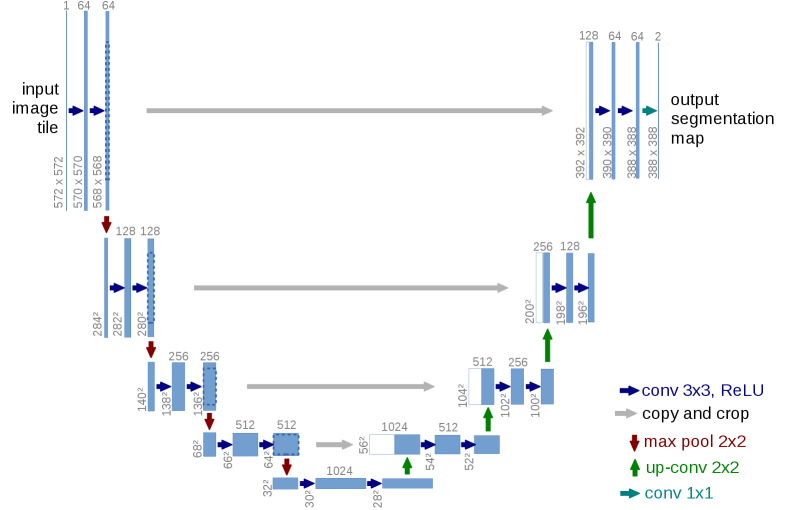
\includegraphics[width=0.92\textwidth]{images/arch_unet2d.png}
    \caption{Kiến trúc U-Net với bốn cấp độ phân giải.}
    \label{fig:unet_architecture}
\end{figure}

Kết nối tắt giúp bảo toàn thông tin không gian nhưng đồng thời có thể truyền cả đặc trưng ít liên quan hoặc nhiễu nền sang bộ giải mã. Attention U-Net giải quyết một phần hạn chế này bằng cách điều chỉnh đặc trưng tại kết nối tắt trước khi thực hiện phép ghép.

% ------------------------------------------------------------
\subsection{Kiến trúc Attention U-Net}
\label{subsec:attention_unet}

Attention U-Net~\cite{oktay2018attentionunet} chèn Cổng chú ý tại các kết nối tắt của U-Net. Mỗi cổng nhận đặc trưng
$\mathbf{x}^{l}$ từ bộ mã hóa và tín hiệu cổng
$\mathbf{g}^{l}$ từ tầng sâu hơn của bộ giải mã.

Hai đặc trưng được chiếu về cùng không gian và kết hợp để tạo bản đồ chú ý:

\begin{equation}
    \mathbf{q}^{l}
    =
    \boldsymbol{\psi}^{l}
    \ast
    \delta
    \left(
        \mathbf{W}^{l}_{x}\ast\mathbf{x}^{l}
        +
        \mathbf{W}^{l}_{g}\ast\mathbf{g}^{l}
        +
        \mathbf{b}^{l}
    \right),
    \label{eq:attention_gate_score}
\end{equation}

trong đó $\delta$ là hàm ReLU,
$\mathbf{W}^{l}_{x}$ và $\mathbf{W}^{l}_{g}$ là các phép chiếu học được. Hệ số chú ý được xác định bởi:

\begin{equation}
    \boldsymbol{\alpha}^{l}
    =
    \sigma
    \left(
        \mathbf{q}^{l}
    \right),
    \label{eq:attention_gate}
\end{equation}

với $\sigma$ là hàm Sigmoid. Đặc trưng tại kết nối tắt được điều chỉnh theo:

\begin{equation}
    \widehat{\mathbf{x}}^{l}
    =
    \boldsymbol{\alpha}^{l}
    \odot
    \mathbf{x}^{l},
    \label{eq:attention_skip}
\end{equation}

trong đó $\odot$ là phép nhân theo phần tử.

Cổng chú ý cho phép bộ giải mã điều chỉnh lượng thông tin nhận từ bộ mã hóa theo vị trí không gian. Tuy nhiên, cả
$\mathbf{x}^{l}$ và $\mathbf{g}^{l}$ đều được hình thành từ ảnh đầu vào; cơ chế không nhận trực tiếp thông tin định hướng của bác sĩ. PGA-UNet mở rộng điểm này bằng cách điều kiện hóa tín hiệu cổng bằng đặc trưng câu nhắc.

\begin{figure}[htbp]
    \centering
    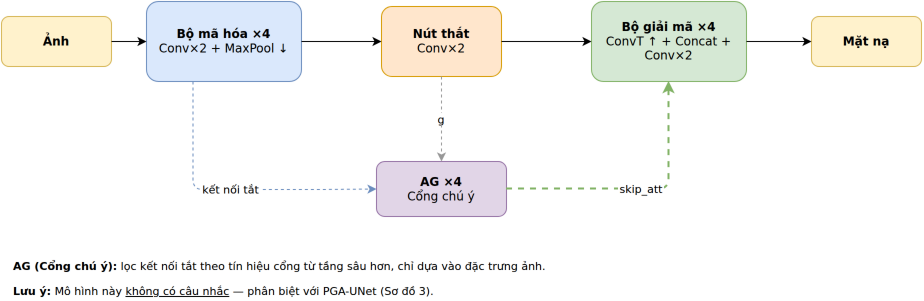
\includegraphics[width=0.98\textwidth]{images/arch_attention_unet2d.png}
    \caption{Kiến trúc Attention U-Net với các cổng chú ý tại các kết nối tắt.}
    \label{fig:attunet_architecture}
\end{figure}

% ------------------------------------------------------------
\section{Biểu diễn và tích hợp câu nhắc trực quan}
\label{sec:prompt}
% ------------------------------------------------------------

Câu nhắc trực quan là thông tin bổ sung do bác sĩ cung cấp để xác định đối tượng hoặc vùng cần phân đoạn. Các dạng câu nhắc phổ biến gồm điểm bấm, nét vẽ, hộp giới hạn và mặt nạ thô. Khóa luận lựa chọn hộp giới hạn vì thao tác này cung cấp đồng thời vị trí và phạm vi tương đối của vùng nghi ngờ nhưng không yêu cầu bác sĩ vẽ chính xác đường biên ở cấp độ điểm ảnh.

% ------------------------------------------------------------
\subsection{Biểu diễn không gian của câu nhắc}
\label{subsec:heatmap}

Hộp giới hạn được xác định bởi tọa độ hai góc đối diện:

\begin{equation}
    \mathbf{B}
    =
    (x_1,y_1,x_2,y_2).
\end{equation}

Để xử lý bằng CNN, hộp có thể được chuyển thành bản đồ không gian
$\mathbf{H}\in[0,1]^{H\times W}$ có cùng kích thước với ảnh đầu vào.

Một cách biểu diễn là phân phối Gaussian hai chiều có tâm tại tâm hình học của hộp:

\begin{equation}
    \mu_x
    =
    \frac{x_1+x_2}{2},
    \qquad
    \mu_y
    =
    \frac{y_1+y_2}{2}.
\end{equation}

Giá trị tại vị trí $(x,y)$ được xác định bởi:

\begin{equation}
    H(x,y)
    =
    \exp
    \left(
        -
        \frac{(x-\mu_x)^2}{2\sigma_x^2}
        -
        \frac{(y-\mu_y)^2}{2\sigma_y^2}
    \right),
    \label{eq:gaussian_heatmap}
\end{equation}

trong đó $\sigma_x$ và $\sigma_y$ điều chỉnh độ phân tán theo hai trục. Bản đồ đạt giá trị lớn nhất tại tâm và giảm dần theo khoảng cách.

Một cách khác là mặt nạ hộp giới hạn nhị phân, trong đó toàn bộ vùng bên trong hộp được gán giá trị 1 và vùng bên ngoài được gán giá trị 0. Biểu diễn này duy trì tín hiệu đồng đều trong hộp nhưng tạo ra thay đổi đột ngột tại đường biên.

PGA-UNet sử dụng dạng kết hợp, gọi là bản đồ nhiệt dạng cao nguyên. Trước tiên, vùng bên trong hộp được gán giá trị 1; sau đó đường biên được làm mềm bằng bộ lọc Gaussian. Cách biểu diễn này duy trì tín hiệu trên toàn bộ vùng được chỉ định và tạo vùng chuyển tiếp liên tục tại đường biên. Công thức và cấu hình cụ thể được trình bày tại Mục~\ref{subsec:plateau_heatmap}, Chương~\ref{Chapter3}.

So với vector tọa độ hoặc biểu diễn nhúng vị trí, bản đồ nhiệt giữ cấu trúc không gian hai chiều và có thể được thay đổi kích thước bằng nội suy để phù hợp với các mức đặc trưng của CNN. Đặc điểm này cho phép câu nhắc được sử dụng tại nhiều tầng thay vì chỉ tại đầu vào.

% ------------------------------------------------------------
\subsection{Điều biến đặc trưng theo tín hiệu điều kiện}
\label{subsec:feature_modulation}

Điều biến đặc trưng là cơ chế thay đổi đặc trưng trung gian dựa trên một tín hiệu điều kiện. Với đặc trưng ảnh $\mathbf{x}$ và điều kiện $\mathbf{z}$, dạng tổng quát có thể được biểu diễn bởi:

\begin{equation}
    \widetilde{\mathbf{x}}
    =
    \boldsymbol{\gamma}(\mathbf{z})
    \odot
    \mathbf{x}
    +
    \boldsymbol{\beta}(\mathbf{z}),
    \label{eq:feature_modulation}
\end{equation}

trong đó $\boldsymbol{\gamma}$ điều chỉnh tỷ lệ và
$\boldsymbol{\beta}$ điều chỉnh độ lệch của đặc trưng.

FiLM~\cite{perez2018film} sử dụng tín hiệu điều kiện để sinh các hệ số điều biến theo kênh. SPADE~\cite{park2019spade} mở rộng ý tưởng này bằng cách sinh tham số điều biến phụ thuộc vị trí không gian từ bản đồ ngữ nghĩa. Hai phương pháp cho thấy tín hiệu điều kiện không nhất thiết chỉ được ghép với đầu vào mà có thể tác động trực tiếp lên đặc trưng trung gian.

PSG trong PGA-UNet thuộc cùng hướng tiếp cận điều biến đặc trưng có điều kiện, nhưng sử dụng bản đồ nhiệt câu nhắc để sinh trọng số khuếch đại theo không gian. Kết nối dư trong PSG duy trì đường truyền đặc trưng gốc, trong khi mô-đun học mức tăng cường phù hợp tại từng tầng mã hóa. Với công thức triển khai của khóa luận, PSG không trực tiếp triệt tiêu đặc trưng nền mà ưu tiên tăng cường vùng được chỉ định bởi câu nhắc. Thiết kế chi tiết được trình bày tại Mục~\ref{subsec:psg}, Chương~\ref{Chapter3}.

% ------------------------------------------------------------
\subsection{Cơ chế chú ý có điều kiện}
\label{subsec:conditioned_attention}

Cách đơn giản nhất để tích hợp câu nhắc vào CNN là ghép bản đồ câu nhắc với ảnh như một kênh đầu vào bổ sung. Tuy nhiên, tín hiệu ghép tại tầng đầu có thể thay đổi hoặc suy giảm qua nhiều phép tích chập và giảm mẫu.

Cơ chế chú ý có điều kiện đưa thông tin câu nhắc trực tiếp vào quá trình tính trọng số chú ý. Về khái niệm, hệ số chú ý tại tầng thứ $l$ được biểu diễn bởi:

\begin{equation}
    \boldsymbol{\alpha}^{l}
    =
    f
    \left(
        \mathbf{x}^{l},
        \mathbf{g}^{l}
        \mid
        \mathbf{H}^{l}
    \right),
    \label{eq:conditioned_attention_general}
\end{equation}

trong đó $\mathbf{x}^{l}$ là đặc trưng bộ mã hóa,
$\mathbf{g}^{l}$ là tín hiệu bộ giải mã và
$\mathbf{H}^{l}$ là biểu diễn câu nhắc tại cùng mức không gian.

Khác với Cổng chú ý nguyên bản chỉ sử dụng đặc trưng nội bộ của mạng, cơ chế có điều kiện cho phép trọng số chú ý phụ thuộc đồng thời vào ảnh và tín hiệu định hướng bên ngoài. CAD trong PGA-UNet hiện thực hóa nguyên lý này bằng cách mã hóa bản đồ nhiệt và dung hợp đặc trưng câu nhắc vào tín hiệu cổng tại từng tầng giải mã. Cấu trúc cụ thể được trình bày tại Mục~\ref{subsec:cad}, Chương~\ref{Chapter3}.

% ------------------------------------------------------------
\section{Các độ đo đánh giá}
\label{sec:metrics}
% ------------------------------------------------------------

Không có một chỉ số nào có thể phản ánh đầy đủ chất lượng phân đoạn trong mọi khía cạnh. Vì vậy, khóa luận dùng kết hợp nhiều độ đo: Dice và IoU để xem mức độ chồng lấp, Precision và Recall để xem xu hướng dự đoán, HD95 để đánh giá sai lệch đường biên và CBL như một chỉ số bổ sung về độ lệch tâm.

% ------------------------------------------------------------
\subsection{Hệ số Dice và chỉ số IoU}
\label{subsec:dice_iou}

Gọi $Y$ là mặt nạ nhãn gốc và $\widehat{Y}$ là mặt nạ dự đoán. Hệ số Dice được xác định bởi:

\begin{equation}
    \operatorname{Dice}
    (Y,\widehat{Y})
    =
    \frac{
        2|Y\cap\widehat{Y}|
    }{
        |Y|+|\widehat{Y}|
    }.
    \label{eq:dice}
\end{equation}

Chỉ số Giao trên Hợp (IoU) được xác định bởi:

\begin{equation}
    \operatorname{IoU}
    (Y,\widehat{Y})
    =
    \frac{
        |Y\cap\widehat{Y}|
    }{
        |Y\cup\widehat{Y}|
    }.
    \label{eq:iou}
\end{equation}

Cả hai chỉ số nhận giá trị trong khoảng $[0,1]$; giá trị càng lớn biểu thị mức độ chồng lấp càng cao. So với Accuracy ở cấp độ điểm ảnh, Dice và IoU ít bị chi phối hơn bởi số lượng lớn điểm ảnh nền.

% ------------------------------------------------------------
\subsection{Precision và Recall}
\label{subsec:precision_recall}

Gọi $TP$ là số điểm ảnh tổn thương được dự đoán đúng, $FP$ là số điểm ảnh nền bị dự đoán nhầm thành tổn thương và $FN$ là số điểm ảnh tổn thương bị bỏ sót.

Precision biểu thị tỷ lệ dự đoán dương tính chính xác:

\begin{equation}
    \operatorname{Precision}
    =
    \frac{TP}{TP+FP}.
    \label{eq:precision}
\end{equation}

Recall biểu thị tỷ lệ vùng tổn thương được phát hiện:

\begin{equation}
    \operatorname{Recall}
    =
    \frac{TP}{TP+FN}.
    \label{eq:recall}
\end{equation}

Mặt nạ dự đoán quá rộng thường có Recall cao nhưng Precision thấp do bao gồm nhiều vùng nền. Ngược lại, mặt nạ quá nhỏ có thể đạt Precision cao nhưng Recall thấp do bỏ sót một phần tổn thương. Vì vậy, hai chỉ số được báo cáo song song với Dice và IoU.

% ------------------------------------------------------------
\subsection{Khoảng cách Hausdorff 95\%}
\label{subsec:hd95}

Dice và IoU đo mức độ chồng lấp diện tích nhưng chưa phản ánh đầy đủ sai lệch đường biên. HD95 đánh giá khoảng cách giữa đường biên dự đoán và đường biên nhãn gốc, đồng thời giảm ảnh hưởng của một số điểm ngoại lai so với khoảng cách Hausdorff cực đại.

Gọi $X$ và $Y$ lần lượt là tập điểm trên đường biên dự đoán và đường biên nhãn gốc. Tập khoảng cách biên hai chiều được xác định bởi:

\begin{equation}
    \begin{split}
    \mathcal{D}(X,Y)
    ={}&
    \left\{
        \min_{y\in Y}d(x,y)
        \mid x\in X
    \right\}
    \\
    &\cup
    \left\{
        \min_{x\in X}d(y,x)
        \mid y\in Y
    \right\},
    \end{split}
    \label{eq:surface_distances}
\end{equation}

trong đó $d(\cdot,\cdot)$ là khoảng cách Euclidean. HD95 là phân vị thứ 95 của tập khoảng cách trên:

\begin{equation}
    \operatorname{HD95}(X,Y)
    =
    \operatorname{Percentile}_{95}
    \left(
        \mathcal{D}(X,Y)
    \right).
    \label{eq:hd95}
\end{equation}

HD95 được báo cáo theo đơn vị điểm ảnh trong khóa luận. Giá trị càng nhỏ cho thấy đường biên dự đoán càng gần đường biên tham chiếu.

% ------------------------------------------------------------
\subsection{Chỉ số định vị tâm CBL}
\label{subsec:cbl}

Bên cạnh các độ đo tiêu chuẩn, khóa luận sử dụng CBL (\textit{Center-Based Localization}) như một chỉ số bổ sung để khảo sát độ lệch tâm giữa mặt nạ dự đoán và nhãn gốc. Chỉ số này đặc biệt hữu ích khi đánh giá mô hình trong kịch bản câu nhắc bị lệch tâm, nhưng không thay thế Dice hoặc HD95.

Với mặt nạ nhị phân không rỗng $M$, tọa độ tâm được xác định bởi:

\begin{equation}
    x_M
    =
    \frac{
        \sum_{x,y}xM(x,y)
    }{
        \sum_{x,y}M(x,y)
    },
    \qquad
    y_M
    =
    \frac{
        \sum_{x,y}yM(x,y)
    }{
        \sum_{x,y}M(x,y)
    }.
    \label{eq:mask_centroid}
\end{equation}

Gọi $(x_p,y_p)$ là tâm mặt nạ dự đoán,
$(x_g,y_g)$ là tâm nhãn gốc và $D_{\mathrm{GT}}$ là độ dài đường chéo của hộp bao nhỏ nhất quanh nhãn gốc. CBL được xác định bởi:

\begin{equation}
    \operatorname{CBL}
    =
    \max
    \left(
        0,\,
        1-
        \frac{
            \sqrt{
                (x_p-x_g)^2+
                (y_p-y_g)^2
            }
        }{
            D_{\mathrm{GT}}
        }
    \right).
    \label{eq:cbl}
\end{equation}

CBL bằng 1 khi hai tâm trùng nhau và giảm dần khi khoảng cách tâm tăng. Việc chuẩn hóa theo $D_{\mathrm{GT}}$ giúp diễn giải sai lệch tương đối theo kích thước tổn thương. Khi mặt nạ dự đoán rỗng, CBL được quy ước bằng 0. Với ảnh có nhiều vùng tổn thương, tâm được tính trên mặt nạ hợp nhất theo phương pháp đánh giá cấp độ ảnh tại Chương~\ref{Chapter4}.

Do CBL là chỉ số bổ sung được sử dụng trong phạm vi khóa luận, kết luận chính về chất lượng phân đoạn vẫn dựa trên các độ đo tiêu chuẩn gồm Dice, IoU, Precision, Recall và HD95.

% ------------------------------------------------------------
\section{Tổng kết chương}
\label{sec:summary_ch2}
% ------------------------------------------------------------

Chương này đã điểm qua các phương pháp phân đoạn tự động, phân đoạn tương tác dựa trên CNN và mô hình nền tảng dựa trên câu nhắc. Từ đó, khóa luận thấy rõ hơn khoảng trống nghiên cứu mà nhóm chúng tôi nhắm tới: nhu cầu về một kiến trúc CNN hạng nhẹ có thể tiếp nhận và giữ thông tin câu nhắc trong suốt quá trình phân đoạn.

Các cơ sở lý thuyết về U-Net, Cổng chú ý, bản đồ nhiệt, điều biến đặc trưng và chú ý có điều kiện là cơ sở để đi đến thiết kế PGA-UNet ở Chương~\ref{Chapter3}. Chương này cũng chốt các độ đo sẽ dùng để đánh giá định lượng mô hình ở Chương~\ref{Chapter4}.
